% Plot für ET3 Übung 8, Vorlesung Prof. Exknowski, digitalisierte Musterlösung leicht verändert
% Stromverlauf i3(t) für -tau < t < 5tau, tau=0,3ms
% i3(t<0) = 0,1A
% t3(t=0) = 0,5A
% i3(t>0) = (0,5A - 0,2A)*e^(-t/tau) + 0,2A
% i3(t>5tau) = 0,2A
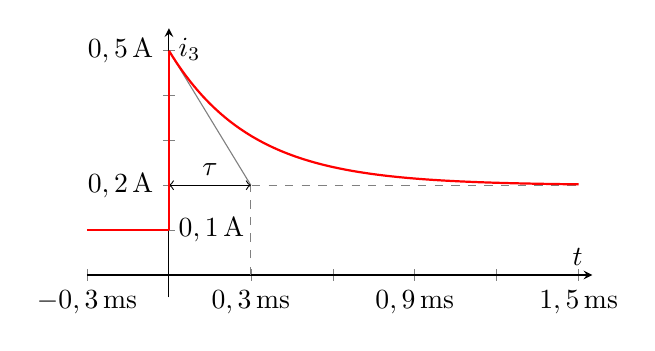
\begin{tikzpicture}
\begin{axis}[
    axis lines=center,
    xlabel={$t$},
    ylabel={$\eci{i_3}$},
    xmin=-0.30, xmax=1.55,
    ymin=-0.05, ymax=0.55,
    xtick distance=0.3, % schluckt das label bei 0, wenn axis lines=center
    ytick distance=0.1, % schluckt das label bei 0, wenn axis lines=center
    xticklabels={,{$-0,3\,\mathrm{ms}$},{$0$}, {$0,3\,\mathrm{ms}$}, , {$0,9\,\mathrm{ms}$}, , {$1,5\,\mathrm{ms}$}},
    yticklabels={,$0$,,{$0,2\,\mathrm{A}$},,,{$0,5\,\mathrm{A}$}},
    grid=none,
    width=8cm,
    height=5cm,
]
    \node at (0,0.1) [right]{$0,1\,\mathrm{A}$};
    \addplot[gray, domain=0:0.3]{(0.2-0.5)/0.3*x+0.5};% Asymptote für t=0, Steigung (i(end)-i(0))/tau
    \addplot[gray, dashed, domain=0:1.5]{0.2};% Asymptote für t>5tau
    \addplot[gray, dashed] coordinates {(0.3,0) (0.3,0.2)};% tau
    \addplot[black, domain=0:0.3, <->]{0.2} node[pos=0.5, above]{$\tau$};% tau
    \addplot[red, thick, domain=-0.3:0]{0.1};% i3(t<0)
    \addplot[red, thick] coordinates {(0,0.1) (0,0.5)};% Sprung bei t=0
    \addplot[red, thick, domain=-0:1.5, samples=100]{(0.5-0.2)*exp(-x/0.3)+0.2};% i3(t>0)
\end{axis}
\end{tikzpicture}
